\documentclass[fleqn,10pt]{wlpeerj}

\usepackage{graphicx}              % to include figures
\usepackage{amsmath}               % great math stuff
\usepackage{amsfonts}              % for blackboard bold, etc
\usepackage{amsthm}                % better theorem environments
\usepackage{listings}
\usepackage{multirow}
\usepackage{hyperref}
\usepackage{parskip}

\title{NxRepair: Error Correction in De Novo Sequence Assembly Using Nextera Mate Pairs}

\author[1]{Rebecca R. Murphy}
\author[2]{Jared O'Connell}
\author[3]{Anthony J. Cox}
\author[4]{Ole Schulz-Trieglaff}
\affil[1]{Illumina Cambridge, Chesterford Research Park, Essex, CB10 1XL}
\affil[2]{Illumina Cambridge, Chesterford Research Park, Essex, CB10 1XL}
\affil[3]{Illumina Cambridge, Chesterford Research Park, Essex, CB10 1XL}
\affil[4]{Illumina Cambridge, Chesterford Research Park, Essex, CB10 1XL}

\keywords{de novo assembly, bioinformatics, error correction, bacteria}

\begin{abstract}
Scaffolding errors and incorrect traversals of the de Bruijn graph during de novo assembly can result in large scale misassemblies in draft genomes. Nextera mate pair sequencing data provide additional information to resolve assembly ambiguities during scaffolding. Here, we introduce NxRepair, an open source toolkit for error correction in de novo assemblies that uses Nextera mate pair libraries to identify and correct large-scale errors. We show that NxRepair can identify and correct large scaffolding errors, without use of a reference sequence, resulting in quantitative improvements in the assembly quality. NxRepair can be downloaded from GitHub; a tutorial and user documentation are also available.
\end{abstract}

\begin{document}

\flushbottom
\maketitle
\thispagestyle{empty}

\section*{Introduction}
De Bruijn Graph construction and traversal is a popular method for de novo genome assembly~\citep{compeau2011}. However, traversal of repeat regions, which tangle the de Bruijn Graph, remains challenging. Read pairs with a large insert size, such as the Illumina Nextera mate pairs can provide additional information for repeat disambiguation. Many assemblers incorporate mate pair insert size information into the assembly and scaffolding process~\citep{Bankevich2012, zerbino2008}, but large scale scaffolding errors can still occur (Fig.~\ref{fig:NxRepair} (A)). 

Error correction in de novo assemblies is a well-studied problem. Recent work, such as the Assemblathon~\citep{Bradnam2013} and GAGE~\citep{Salzberg2012} collaborations, compare the quality of assemblies prepared by various assemblers. A Bayesian method of assembly quality evaluation also exists~\citep{Ghodsi2013}. Several recent papers have developed error identification and correction methods. The A5 Assembly Pipeline~\citep{Coil2014} includes an error detection and rescaffolding step and two new tools, REAPR~\citep{Hunt2013} and ALE~\citep{Clark2013} use read pair data to identify misassemblies. A similar tool is currently under development at the Broad Institute~\citep{pilon2014}. However with the exception of ALE, which is no longer actively maintained, these tools are not optimised to use mate pair information.  

Here we introduce NxRepair, an assembly error detection tool that can identify the most serious misassemblies, without using a reference sequence, by examining the distribution of Nextera mate pair insert sizes. NxRepair specifically targets the most serious misassemblies by identifying regions with a high number of anomalous insert sizes, breaking the scaffold and optionally trimming out the misassembled region. NxRepair is complementary to existing tools, as it specifically uses Nextera mate pair information to find the largest and most serious misassemblies.

\begin{figure*}
\centerline{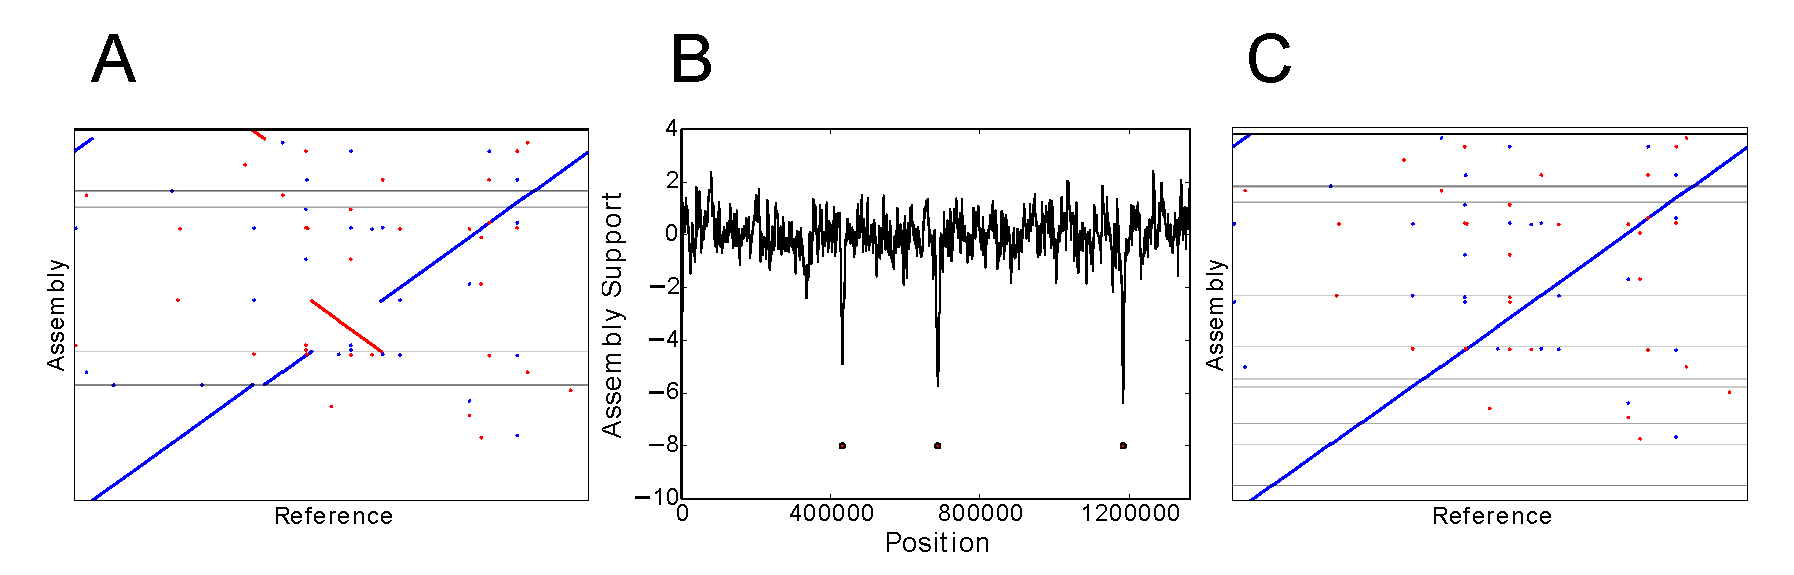
\includegraphics[width=0.8\textwidth]{fig1_nxrepair.pdf}}
\caption{Using NxRepair to remove large misassemblies. (A) A de novo assembly of the Mycobacterium tuberculosis genome contains several large misassemblies. (B) Low support for the assembly is identified in two regions using NxRepair. (C) Breaking the contigs at the identified positions resolves the most significant misassemblies. In (A) and (C), horizontal lines demarcate contig boundaries.}\label{fig:NxRepair}
\end{figure*}

\section*{Implementation}
\subsection*{Statistical Analysis of Mate Pair Insert Sizes}
Nextera mate pair libraries are prepared to have a certain insert size, typically between 1 and 10 kb. When the mate pairs used to prepare an assembly are aligned back to the assembly, large misassemblies result in unusual insert sizes and read orientations. We model this using a two-component mixture distribution. The first component of this mixture is the insert size distribution of correctly aligned mate pairs.  We model the distribution of insert sizes, $Y$, as a normal distribution with mean $\hat{\mu}$ and standard deviation $\hat{\sigma}$: $Y \sim N(\hat{\mu},\hat{\sigma}^2).$ We estimate $\hat{\mu}$ and $\hat{\sigma}$ for the entire genome by aligning reads back to the assembly and using robust estimators (see below). The second component, defined as a uniform distribution across the contig size $U(0,L)$ for a contig of length $L$, captures anomalous insert sizes.

To calculate the degree of support for the assembly at each site across a contig, NxRepair retrieves all mate pairs spanning a window of size `window' at position $i$ on the contig. We define a latent indicator variable $X_l\in\{0,1\}$ for each pair of reads, $l$, which takes the value $1$ if the insert size came from the null distribution, and $0$ otherwise. Within each window queried, the probability that each retrieved read, $r_l$ is drawn from the null distribution is given by:

\begin{eqnarray} P(X_l=x|Y_l)& =& \frac{P(X_l=x)(Y_l|X_l=x)}{\sum_{k=0}^1P(X_l=k)(Y_l|X_l=k)}\\
  & =& \frac{\pi_x(Y_l|X_l=x)}{\sum_{k=0}^1 \pi_k(Y_l|X_l=k)}
\label{eq:posterior}  
\end{eqnarray}

where $Y_l$ is the insert size of read pair $l$, $\pi_x$ is the user defined prior probability of class $x$ and $\pi_1 + \pi_0 = 1$. The default value of $\pi_0$ is 0.01 (see table~\ref{tab:parameters}), meaning that in the absence of any insert size information, 99 \% of read pairs are expected to arise from the null distribution.  

Within each window, the total support for a correct assembly at position $i$ can be calculated as:

\begin{equation}
D_i = \sum_{l=1}^N P(X_l=1|Y_l)\cdot C_l
\end{equation}

where the summation is over all read pairs aligning across position $i$ and $C_l$ is an indicator variable, reporting pairing orientation:

\begin{equation}
    C_l=
    \begin{cases}
      1, & \text{if}\ \text{mate pairs have correct orientation and strand alignment} \\
      0, & \text{otherwise}
    \end{cases}
  \label{eq:C}
  \end{equation}

Within each contig, the contig assembly support mean $\mu_D$ and variance $s_D$ are calculated from all reads aligning to the contig,
\begin{equation}
\hat{\mu}_D = \frac{\sum_{l=1}^N D_l}{N} \qquad s_D = \frac{\sum_{l=1}^N \sqrt{(D_l - \hat{\mu})^2}}{N}
\label{eq:contigD}
\end{equation}

Using these values, the Z-score $z_l$ within each queried interval is calculated as: 

\begin{equation}
z_l = \frac{D_l - \hat{\mu}_D}{s_D}
%\hat{\mu} = \frac{\sum_l^N D_l}{N} \qquad \s = \frac{\sum_l^N \sqrt{(D_l - \hat{\mu})^2}}{N}
\label{eq:zscore}
\end{equation}

A misassembly is identified if $z_l < T$ for a user-defined threshold $T$ (default value -4). This threshold describes the number of standard deviations below the mean assembly support that is required to identify an anomaly. The default value of -4 will flag only positions whose assembly support is less than four standard deviations below the mean level of support. As the parameters of the distribution are derived from the properties of the assembly, this is robust to variation in coverage, contig size and other assembly properties.

\subsection*{Global Assembly Parameters}
NxRepair identifies misassemblies by identifying regions where the mate pair insert size distribution differs significantly from the insert size distribution across the entirety of the de novo assembly. Consequently, it is necessary to have a robust estimate of the global mate pair insert size distribution. For calculation of population statistics, mate pairs that align to different contigs are excluded, as are mate pairs with an incorrect strand or pairing orientation, pairs whose mapping quality falls below a user specified threshold, and pairs whose insert size exceed 30 Kb (approximately 10 times the mean insert size). The global mean $\hat{\mu}$ and median absolute deviation $\text{MAD}$ are calculated across all contigs in the assembly as:

\begin{equation}
\hat{\mu} = \frac{\sum_{l=1}^N Y_l}{N} \qquad \text{MAD} = \text{median}(|Y_l - \text{median}(Y_l)|)
\label{eq:global}
\end{equation}

where $Y_l$ is the insert size of the $l$th of $N$ reads with correct pairing behaviour. The standard deviation was then calculated from the MAD, using:

\begin{equation}
\hat{\sigma} = K \cdot \text{MAD}
\label{eq:mad_to_sigma}
\end{equation}

for $K = 1.4826$

These were then used as the parameters of the null distribution, as described in the main paper.

\subsection*{Interval Tree Construction}
To facilitate rapid lookup of mate pair properties, we construct an interval tree~\citep{cormen2009} for each contig in the de novo assembly. An interval tree is a datastructure that facilitates $O(\text{log} n + m)$ lookup of intervals that span a given point or interval, for $n$ total entries and $m$ spanning entries. The interval tree contains the start and end positions of each mate pair aligned to that contig, as well as an flag variable indicating whether that mate pair had correct strand and pairing orientation. Mate pairs where the two reads align to different contigs were excluded. This allows NxRepair to rapidly query positions across a contig to discover the insert size distribution at the queried position.  

\subsection*{Misassembly Location and Contig Breaking}
To improve the quality of the de novo assembly, a contig is broken into two separate pieces at the site of a misassembly and the broken ends of the two new contigs trimmed by a user defined length (default 4 Kb) to remove the misassembled region. To prevent excessive clipping, misassemblies separated by less than the trimming distance are grouped together, the contig is broken at the start and end of the misassembled region and the misassembled section is discarded. Low-scoring regions within the trimming distance of the ends of contigs are not considered misassemblies, as the high proportion of mate pairs aligning here whose mate maps to a different contig reduces the number of pairs under consideration and hence lowers the observed Z-score.

\subsection*{Availability and Dependencies}
NxRepair is available for free anonymous download from the Python Package Index (PyPI) here: \url{:https://pypi.python.org/pypi/nxrepair}.
The source code, written in python is hosted on GitHub: \url{https://github.com/rebeccaroisin/nxrepair}.
A full tutorial and API can be found on ReadTheDocs: \url{http://nxrepair.readthedocs.org/en/latest/}.

NxRepair makes use of several further open source libraries, specifically:

\begin{itemize}
\item[] Numpy~\citep{numpy} (\url{http://www.numpy.org/})
\item[] Scipy~\citep{scipy} (\url{http://www.scipy.org/})
\item[] Matplotlib~\citep{Hunter2007} (\url{http://matplotlib.org/})
\item[] Pysam (\url{https://pypi.python.org/pypi/pysam}), the python wrapper for Samtools
\item[] Samtools~\citep{li2009} (\url{http://samtools.sourceforge.net/})
\end{itemize}

We installed the numpy, scipy and matplotlib libraries via Anaconda (\url{https://store.continuum.io/cshop/anaconda/}).

We have used the Interval Tree implementation from the bx-python library (\url{https://bitbucket.org/james_taylor/bx-python/wiki/Home}).   

\section*{Materials and Methods}
\subsection*{Data}
Nine bacterial genomes were prepared according to the Nextera mate pair protocol and sequenced in a single MiSeq run using $2 \times 151$ bp reads. The genomes sequenced are shown in Table~\ref{data-description}. Reads were trimmed using the MiSeq inbuilt trimmer. The untrimmed reads are available from BaseSpace via \url{https://basespace.illumina.com/s/TXv32Ve6wTl9} (free registration required). Note that only these Nextera mate pair libraries were used. No additional single end or paired end libraries were required. 

\begin{table}[]
\begin{center}
{\begin{tabular}{lllllll}\hline
 & \multicolumn{2}{l}{Before NxRepair} & \multicolumn{4}{l}{After NxRepair} \\\hline
Genome & No. & NGA50 & No. & NGA50 \\\midrule
Bcer & 3 & 1157404 & 3 & 1157404 \\
EcDH & 8 & 576143 & 8 & 576143 \\
EcMG & 2 & 640732 & 2 & 640732 \\
List & 0 & 1496615 & 0 & 1496615 \\
Meio & 0 & 3095733 & 0 & 3095733 \\
ped & 6 & 1269259 & 0 & 1269259 \\
pneu & 7 & 577220 & 6 & 577220 \\
Rhod & 9 & 3181390 & 9 & 3181390 \\
TB & 70 & 184170 & 66 & 158885 \\\hline
\end{tabular}}{}
\end{center}
\caption{Number of large misassemblies and NGA50 as reported by QUAST before and after NxRepair correction. \label{tab:improvement}}
\end{table}  

\subsection*{Performance Optimisation}
\subsubsection*{ROC Plots}
To optimimse the threshold in $Z$ below which to identify a misassembled region, we prepared ROC plots, varying the threshold value, $T$, in steps of 1 between -10 and 0. 

As misassemblies are identified as point errors, but NxRepair identifies the region spanned by a misassembly, we needed a method to correctly compare the sites of true misassemblies with those identified by NxRepair. To make this comparison, we divided each contig of the assembly into short stretches of 1 Kb length. We then prepared an array, $A_{Nx}$ of size $\frac{L}{1000}$ for contig length $L$, corresponding to misassemblies identified by NxRepair. $A_{Nx}$ was filled as follows:

\begin{equation}
    A_{Nx}=
    \begin{cases}
      1, & \text{if}\ \text{NxRepair identified a misassembly in stretch $i$} \\
      0, & \text{otherwise}
    \end{cases}
  \label{eq:found}
\end{equation}

To prepare the ROCs each position $i$ in $A_{Nx}$ was labeled as true positive (TP) if $A_{Nx}[i] = 1$ and a true misassembly fell within it, true negative (TN) if $A_{Nx}[i] = 0$ and no true misassembly occurred within the interval, false positive (FP) if $A_{Nx}[i] = 1$ but no true misassembly had occurred, or false negative (FN) if $A_{Nx}[i] = 0$ but the interval contained a true misassembly. The true positive rate (TPR) and false positive rate (FPR) were then calculated as follows:

\begin{equation}
\text{TPR} = \frac{\text{TP}}{\text{TP} + \text{FN}} \qquad \text{FPR} = \frac{\text{FP}}{\text{FP} + \text{TN}}
\label{eq:tpr}
\end{equation}

Based on the resultant ROC plots, shown in Figure~\ref{fig:ROCs}, a threshold in $Z$ of -4 was found to optimise the true positive: false positive ratio. This threshld was used for all subsequent analyses. 

\begin{figure}
\centerline{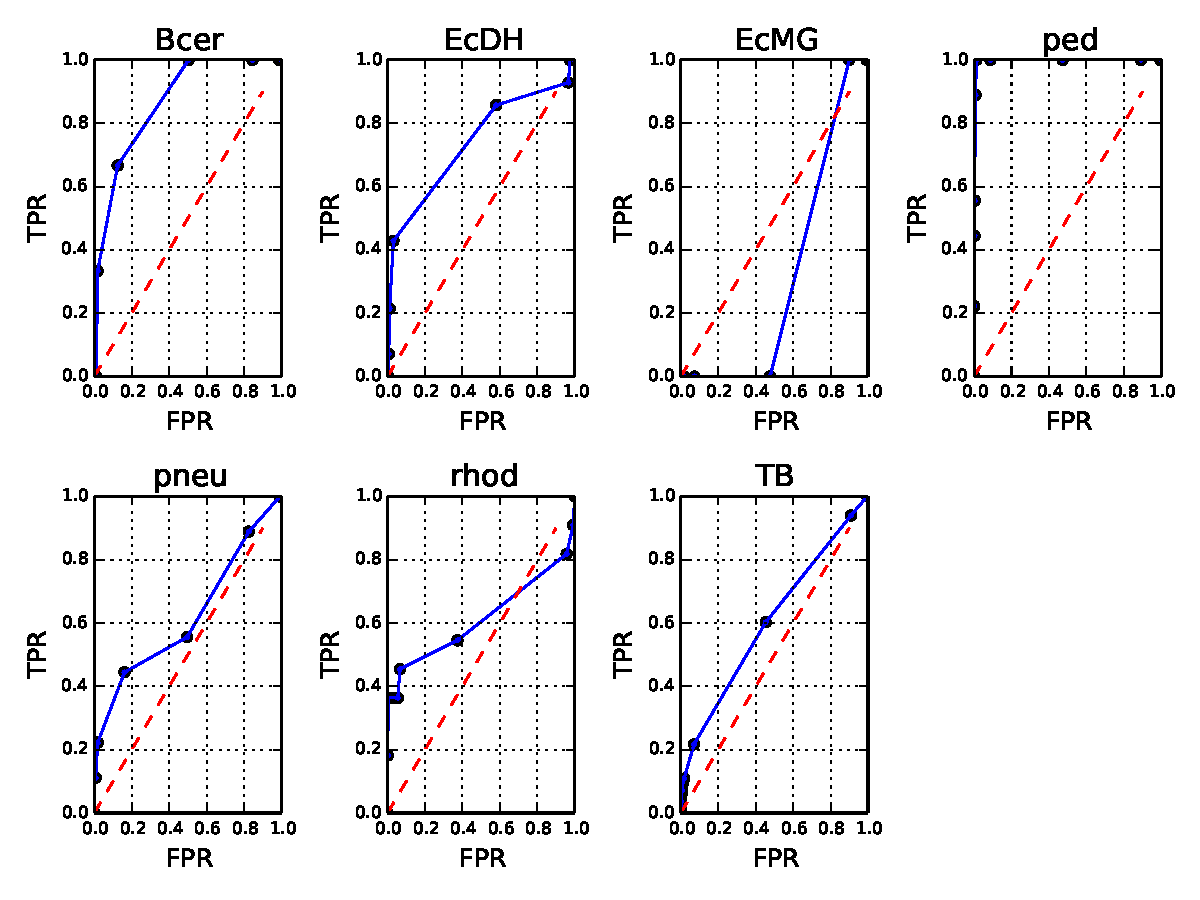
\includegraphics[width=0.8\textwidth]{allROC_extensive.pdf}}
\caption{ROC plots for the seven genomes containing misassemblies.\label{fig:ROCs}}
\end{figure}

\subsubsection*{Profiling}
Performance analysis was performed on a single core with 8 GB RAM available. Runtime analysis was performed using the python cProfile module. The memoryprofiler python module was used to analyse memory usage.

\subsection*{Workflow Pipeline}
De novo assemblies were prepared using the SPAdes Assembler, version 3.1.1~\citep{Bankevich2012}:

\texttt{spades.py -k 21,33,55,77 -t 4 --careful \\ --hqmp1-12 bacteria.fastq.gz  --hqmp1-fr -o assembly}

The initial assembly quality was evaluated using QUAST~\citep{gurevich2013} to align the de novo assembly to a reference genome:

\texttt{python quast.py -o results\_sample -t 16 \\  -R ref/reference.fna sample\_new.fasta }

Following assembly, the mate pair reads were aligned back to the de novo assembly using BWA-MEM~\citep{li2013}. A sorted BAM file of the resulting alignment was then prepared using SAMtools~\citep{li2009}: 

\texttt{bwa index sample/scaffolds.fasta}

\texttt{bwa mem sample/scaffolds.fasta -p bacteria.fastq.gz | samtools view -bS - |  samtools sort - sample}

\texttt{samtools index sample.bam}

We identified misassemblies using NxRepair as follows:

\texttt{python nxrepair.py sample.bam   sample/scaffolds.fasta sample\_scores.csv  sample\_new.fasta -img\_name sample\_new}


The default parameters used and their meanings are shown in Table~\ref{tab:parameters}. These have been optimised for Illumina Nextera mate pair libraries with a mean insert size of approximately 3 Kb. For mate pair libraries with a much larger (smaller) insert size, the maxinsert and trim parameters may need to be increased (decreased).

\begin{table}
\begin{center}
\begin{tabular}{|c|c|p{8cm}|}
    \hline
    Parameter & Default Value & Meaning \\ \hline
    imgname & None & Prefix under which to save plots. \\
    maxinsert & 30000 &  Maximum insert size, below which a read pair is included in calculating population statistics.\\
    minmapq & 40 & Minimum MapQ value, above which a read pair is included in calculating population statistics.\\
    minsize & 10000 & Minimum contig size to analyse.\\ 
    prior & 0.01 & Prior probablility that the insert size is anomalous.\\
    stepsize & 1000 & Step-size in bases to traverse contigs.\\
    trim & 4000 & Number of bases to trim from each side of an identified misassembly.\\
    T & -4.0 & Threshold in Z score (number of standard deviations from the mean) below which a misassembly is called.\\
    window & 200 & Window size across which bridging mate pairs are evaluated.\\ \hline
\end{tabular}
\end{center}
\caption{NxRepair Parameters \label{tab:parameters}}
\end{table}

Finally we used QUAST~\citep{gurevich2013} to evaluate the assembly quality following NxRepair by aligning the de novo assembly to a reference genome as described above.


\section*{Results and Discussion}
We used NxRepair to correct de novo assemblies from nine bacterial genomes. The genomes used are described above. Mate pair reads were trimmed, assembled using the SPAdes assembler (version 3.1.1)~\citep{Bankevich2012} and then aligned back to the assembled scaffold using BWA-MEM~\citep{li2013}. We used QUAST~\citep{gurevich2013} to evaluate the assembly quality before and after NxRepair correction by aligning to an appropriate reference genome. For all NxRepair analyses, the default parameters, shown in Table~\ref{tab:parameters} were used. Fig.~\ref{fig:NxRepair} (A) shows a misassembled genome that contained several scaffolding errors identified by NxRepair (Fig.~\ref{fig:NxRepair} (B)). Following NxRepair correction, the most significant structural misassemblies were resolved (Fig.~\ref{fig:NxRepair} (C)). The improvement following NxRepair correction is shown for all nine genomes in Table~\ref{tab:improvement}. For two assemblies, errors were removed without reducing NGA50; for one genome, errors were removed but NGA50 was slightly reduced; for five genomes, two of which contained no large errors, no errors were found and the assembly was unchanged.

Finally, we plotted the NGA50 value as calculated by QUAST against the NA50, before and after NxRepair correction, to demonstrate that we have not reduced the assembly quality. This is shown in Figure~\ref{fig:NGA50}. We note that in the case of the TB genome, the NGA50 was slightly reduced by NxRepair correction. Manual inspection of the correction sites revealed that one of the misassemblies reported by nxrepair was a join between two contigs which consisted of a gap of over 2 Kb bridged by very few mate pairs. This join is reported as correct by Quast, but has only little support from the read data. We fail to correct some misassemblies because they do not exhibit a signal given the wide insert size distribution of the Nextera mate pairs.

\begin{figure}
\centerline{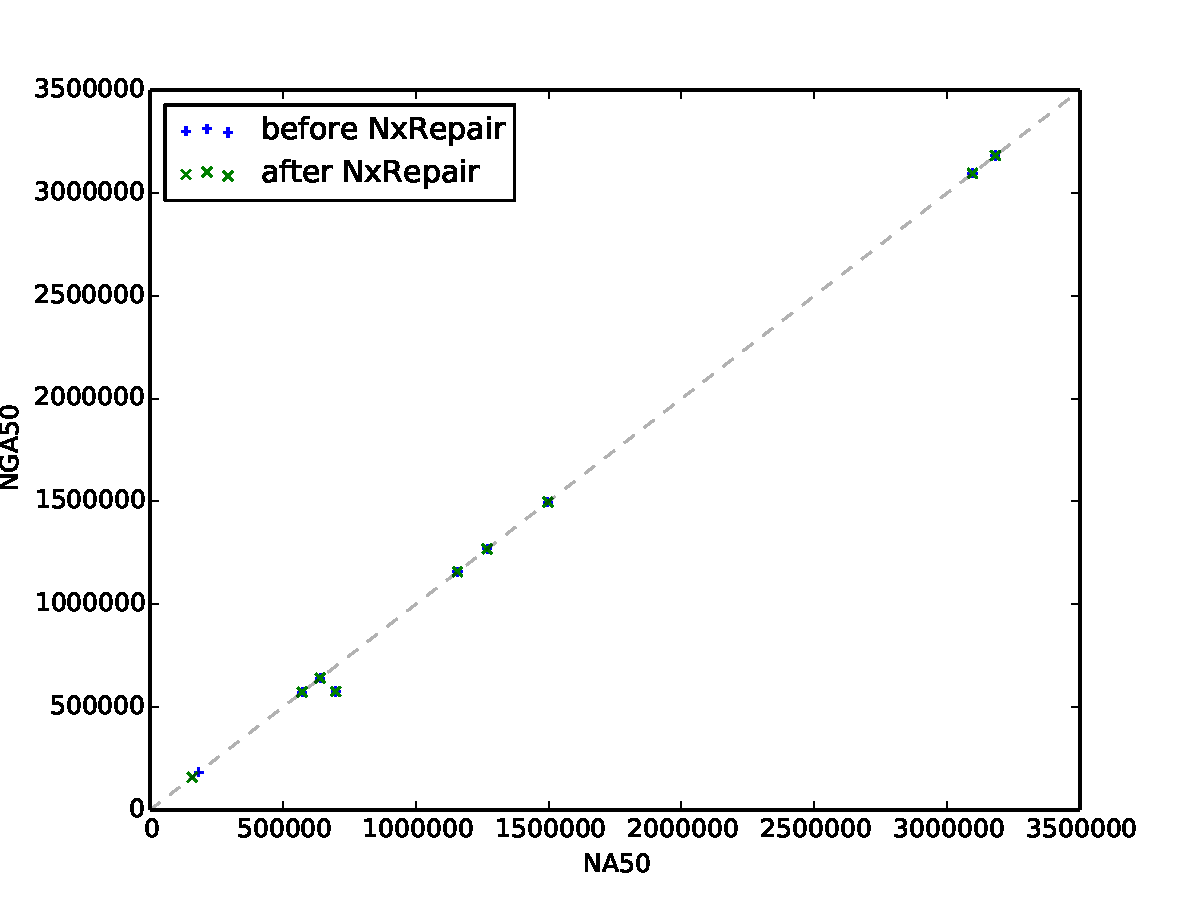
\includegraphics[width=0.8\textwidth]{ng50.pdf}}
\caption{Plot of NGA50 vs NA50 for each genome before and after NxRepair correction.\label{fig:NGA50}}
\end{figure}

\subsection*{Performance}
We evaluated the runtime and peak memory usage of NxRepair on each of the nine genomes analysed. The results are shown in table~\ref{tab:performance}. The most memory and computationally intensive part of the NxRepair analysis is construction of the interval trees. The size of each interval tree is dependent on the contig size. Consequently, we expect both runtime and memory usage to scale with the size of the largest contig. 

\begin{table}
\begin{center}
\begin{tabular}{|c|c|c|}
    \hline
    Bacterium & Total Time (s) & Memory Usage (MiB) \\ \hline
    Bcer & 78 & 271 \\
    EcDH & 123 & 444 \\
    EcMG & 70 & 260 \\
    list & 97 & 383 \\
    meio & 259 & 565 \\
    ped & 123 & 417 \\
    pneu & 59 & 227 \\
    rhod & 190 & 463 \\
    TB & 155 & 411 \\ 
    \hline
\end{tabular}
\end{center}
\caption{NxRepair performance analysis. \label{tab:performance}}
\end{table}

\begin{table}[h]
  \centering
\resizebox{\textwidth}{!}{
  \begin{tabular}{ll}
    \hline
    \textbf{Abbreviation:}             &    Bcer \\
    \textbf{Bacteria:}                 &    \emph{Bacillus cereus ATCC 10987} \\
    \textbf{Accession ID:}  &  NC\_003909, NC\_005707 \\ 
    \textbf{NCBI FTP:}                 &    \url{ftp.ncbi.nih.gov/genomes/Bacteria/Bacillus\_cereus\_ATCC\_10987\_uid57673/} \\
    \hline
    \textbf{Abbreviation:}             &    EcDH \\ 
    \textbf{Bacteria:}                 &    \emph{Escherichia coli str. K-12 substr. DH10B}\\ 
    \textbf{Accession ID:}              &    NC\_010473 \\ 
    \textbf{NCBI FTP:}     &    \url{ftp.ncbi.nih.gov/genomes/Bacteria/Escherichia\_coli\_K\_12\_substr\_\_DH10B\_uid58979/}\\
    \hline
    \textbf{Abbreviation:}             &   EcMG \\
    \textbf{Bacteria:}                 & \emph{Escherichia coli str. K-12 substr. MG1655}\\
    \textbf{Accession ID:}            & NC\_000913    \\ 
    \textbf{NCBI FTP:}       & \url{ftp.ncbi.nih.gov/genomes/Bacteria/Escherichia\_coli\_K\_12\_substr\_\_MG1655\_uid57779/}\\
    \hline
    \textbf{Abbreviation:}             &   list\\ 
    \textbf{Bacteria:}                 &\emph{Listeria monocytogenes}\\  
\textbf{Accession ID:}              & NC\_003210 \\ 
\textbf{NCBI FTP:}     & \url{ftp.ncbi.nih.gov/genomes/Bacteria/Listeria\_monocytogenes\_EGD\_e\_uid61583/}\\
\hline
\textbf{Abbreviation:}             &  meio \\ 
\textbf{Bacteria:}                 &\emph{Meiothermus ruber DSM 1279}\\ 
\textbf{Accession ID:}             &NC\_013946 \\ 
\textbf{NCBI FTP:}      & \url{ftp.ncbi.nih.gov/genomes/Bacteria/Meiothermus\_ruber\_DSM\_1279\_uid46661/}\\
   \hline
\textbf{Abbreviation:}             &  ped \\
\textbf{Bacteria:}                 &\emph{Pedobacter heparinus DSM 2366}\\
\textbf{Accession ID:}                 & NC\_013061 \\ 
\textbf{NCBI FTP:}  & \url{ftp.ncbi.nih.gov/genomes/Bacteria/Pedobacter\_heparinus\_DSM\_2366\_uid59111/}\\
   \hline
\textbf{Abbreviation:}             &   pneu \\
\textbf{Bacteria:}                 & \emph{Klebsiella pneumoniae subsp. pneumoniae MGH 78578}  \\
\textbf{Accession ID:}              & NC\_009648, NC\_009649, NC\_009650, NC\_009651, NC\_009652, NC\_009653 \\ 
\textbf{NCBI FTP:}     & \url{ftp.ncbi.nih.gov/genomes/Bacteria/Klebsiella\_pneumoniae\_MGH\_78578\_uid57619/}\\
   \hline
\textbf{Abbreviation:}             &  rhod \\ 
\textbf{Bacteria:}                 &\emph{Rhodobacter sphaeroides 2.4.1}\\ 
\textbf{Accession ID:}                 &NC\_007488, NC\_007489, NC\_007490, NC\_007493, NC\_007494, NC\_009007, NC\_009008\\ 
\textbf{NCBI FTP:}  & \url{ftp.ncbi.nih.gov/genomes/Bacteria/Rhodobacter\_sphaeroides\_2\_4\_1\_uid57653/}\\ 
   \hline
\textbf{Abbreviation:}             &  TB \\
\textbf{Bacteria:}                 & \emph{Mycobacterium tuberculosis H37Ra}\\ 
\textbf{Accession ID:}               &NC\_009525 \\ 
\textbf{NCBI FTP:}    & \url{ftp.ncbi.nih.gov/genomes/Bacteria/Mycobacterium\_tuberculosis\_H37Ra\_uid58853/}\\ 
   \hline
  \end{tabular}
}
  \caption{Summary of bacteria analysed and the relevant NCBI information on their reference genomes. There were two repeats of each strain. All 18 samples were prepared with the Nextera mate pair protocol and sequenced in a single MiSeq run using $2 \times 151$ bp reads. The untrimmed reads we used as input to NxTrim (3.9Gbp in all) are available from BaseSpace via \url{https://basespace.illumina.com/s/TXv32Ve6wTl9} (free registration required).\label{data-description}}
\end{table}

\section*{Conclusions}
NxRepair is a simple error correction module that can be used to identify and remove large scale errors from de novo assemblies using Nextera mate pair reads. We evaluated NxRepair using nine bacterial genomes, showing that of the seven genomes containing misassemblies, six could be improved by NxRepair correction. NxRepair is freely available online and can be run with a single call from the command line, making it an attractive option for improving assembly quality.

\section*{Acknowledgments}


\bibliography{detecting_large_missassemblies}
%\bibliographystyle{unsrt}

\end{document}
